\section{Remapping Routing Events}
\label{sec:patching}

Routing events impact multiple paths in the Internet. Current
monitoring techniques monitor paths independently. Detecting
a routing event on one Internet paths does not trigger any action on
other possibly-impacted paths.  This approach (i) leads to outdated
routing information (as we do not remap paths that have possibly
changed due to the routing events) and (ii) prevents us from
observing the extent of a routing event (as other routing events
might happen before we remap all routes impacted by the first one).
In this section we investigate whether we can use information about
a just-remapped change to quickly detect and remap changes the
underlying routing event caused on other paths.  Our goal is to
develop techniques to efficiently (using few probes) identify and
remap paths impacted by a routing event.

\newcommand{\lczd}{\ensuremath\mathrm{\textsc{lczd}}}

We define a \emph{local change zone domain}, denoted $\lczd(r')$,
for a change detected at radius $r'$ as the hops removed from the
previous path, $p_{i-1}$, around $r'$. More formally, if $r_d$ and
$r_c$ are the radii of the divergence and convergence hops,
respectively, and if $r^\prime_d = p_{i-1}\langle p[r_d]\rangle$ and
$r^\prime_c = p_{i-1}\langle p[r_c]\rangle$ are the radii of the
divergence and convergence hops on the previous route, then
$\lczd(r')$ is defined as the set of hops in $p_{i-1}$ between
$r^\prime_d$ and $r^\prime_c$, i.e., $\lczd(r') = \{p_{i-1}[x]
\mid{} r^\prime_d < x < r^\prime_c\}$.

We extended \dtrack{} to evaluate techniques for remapping paths
after detection of a routing event.  Upon detecting a path change at
radius $r'$ on path $p_{i-1}$ (i.e., $p[r'] \ne p_{i-1}[r']$),
\dtrack{} immediately queues path $p_{i-1}$ to be remapped
(remapping starts immediately if there are no ongoing remaps).
After remapping of path $p_{i-1}$ is complete, we compute
$\lczd(r')$.  Our extended \dtrack{} then queues all (other)
\emph{overlapping paths} $q$ who intersect $\lczd(r')$, i.e., $q\,
\cap\,\lczd(r') \ne \emptyset$, for remapping.  We use this data to
study when and how overlapping paths change.

Figure~\ref{fig:overlap.delay.cdf} shows the CDF, over all detected
path changes, of the approximate time it takes to remap all
overlapping paths.  Because we remap overlapping paths within
a short period, there is a lower probability that subsequent routing
events will happen while remap is ongoing.
Figure~\ref{fig:overlap.quantity.cdf} shows the CDF, over all
detected path changes, of the fraction of overlapping paths (i.e.,
fraction of other paths that overlap with local change zone
domains).  We observe that TODO.

For each detected path change, we check which of the overlapping
paths have also changed.  Figure~\ref{fig:overlap.change.prob} shows
the fraction of overlapping paths that have changed, grouping
overlapping paths by the fraction of the local change zone domain
that intersects the overlapping paths, i.e.,
$|q\,\cap\,\lczd|\div|\lczd|$.  We note that as overlapping paths
have more in common with the local change zone domain, the higher
the probability that the overlapping path will change.  We also find
that paths that have more in common with the path where the change
was detected have even higher probability of changing (not shown
\ed{@elverton: but please plot so we can see}).

We now want to find a way to identify whether an overlapping path
has changed (or remained stable).  Let $\lczd'$ denote the local
change zone domain for an overlapping path that has changed, and let
$I = \lczd\,\cap\,\lczd'$ denote the \emph{intersection} of the
local change zone domains for the path where the routing event was
first detected ($\lczd$) and an overlapping path ($\lczd'$).
Figure~\ref{fig:lczd.intersection} shows the distribution of the
size of the intersection in local change zone domains $I$ by the
size of local change zone domain where the change was detected,
i.e., $|I|\div|\lczd|$.  The distribution shows that the
intersection $I$ is usually the same size as $\lczd$, meaning that
when an overlapping path has changed, probing almost any hop in
$\lczd'$ will detect the change (if there is one).  We also looked
at where the intersection $I$ is located compared to $\lczd$.  We
find that XX\% of the intersections $I$ are at the start of the
local change zone (i.e., $r_d + 1$), YY\% of the intersections $I$
are at the end of the local change zone (i.e., $r_c - 1$), and that
only ZZ\% of the intersections do are in neither extreme of the
change zone.

\begin{figure*}[t]
\begin{center}
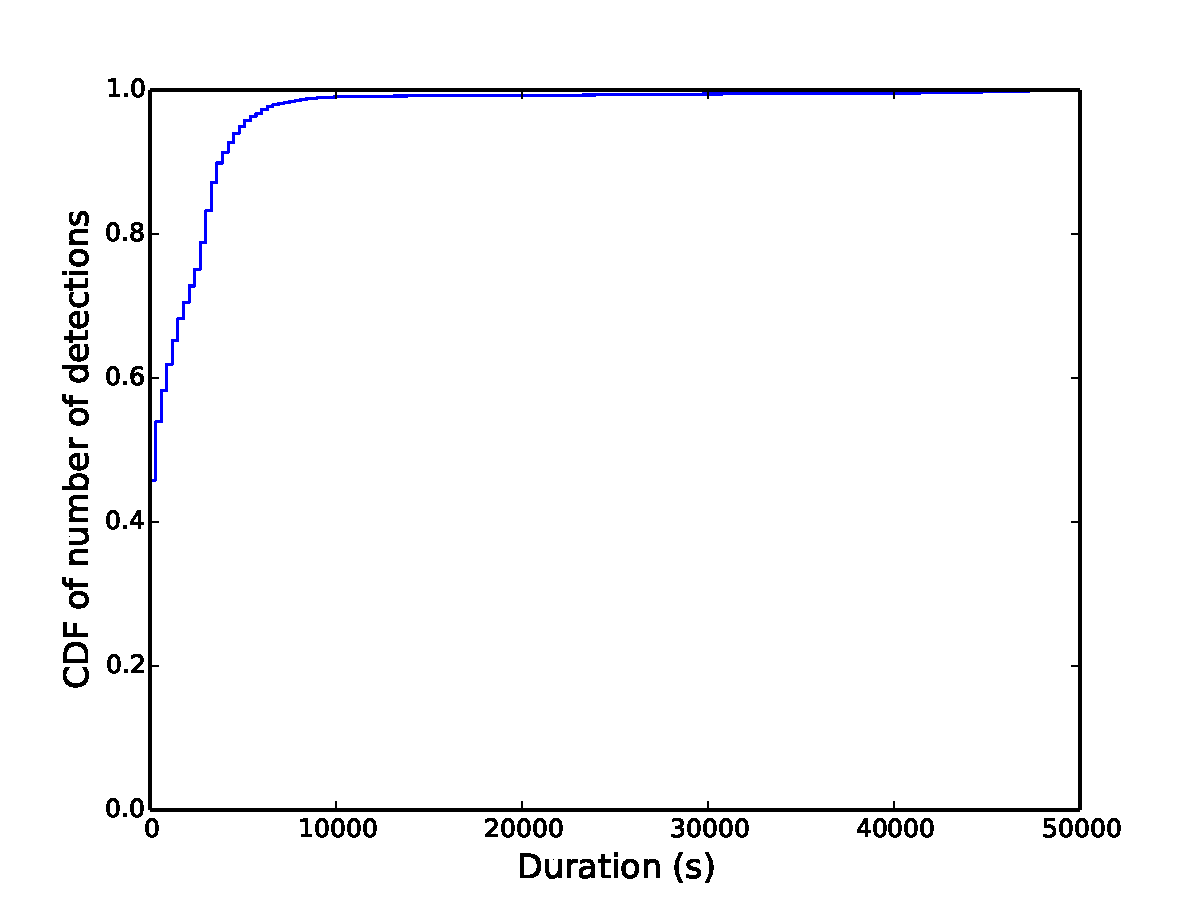
\includegraphics[width=0.8\columnwidth]{figs/patching/durationdetection.pdf}
\caption{CDF of detection duration to remap overlappinh routes. }
\label{fig:branch.acc}
\end{center}
%
\end{figure*}
%
\begin{figure*}[t]
\begin{center}
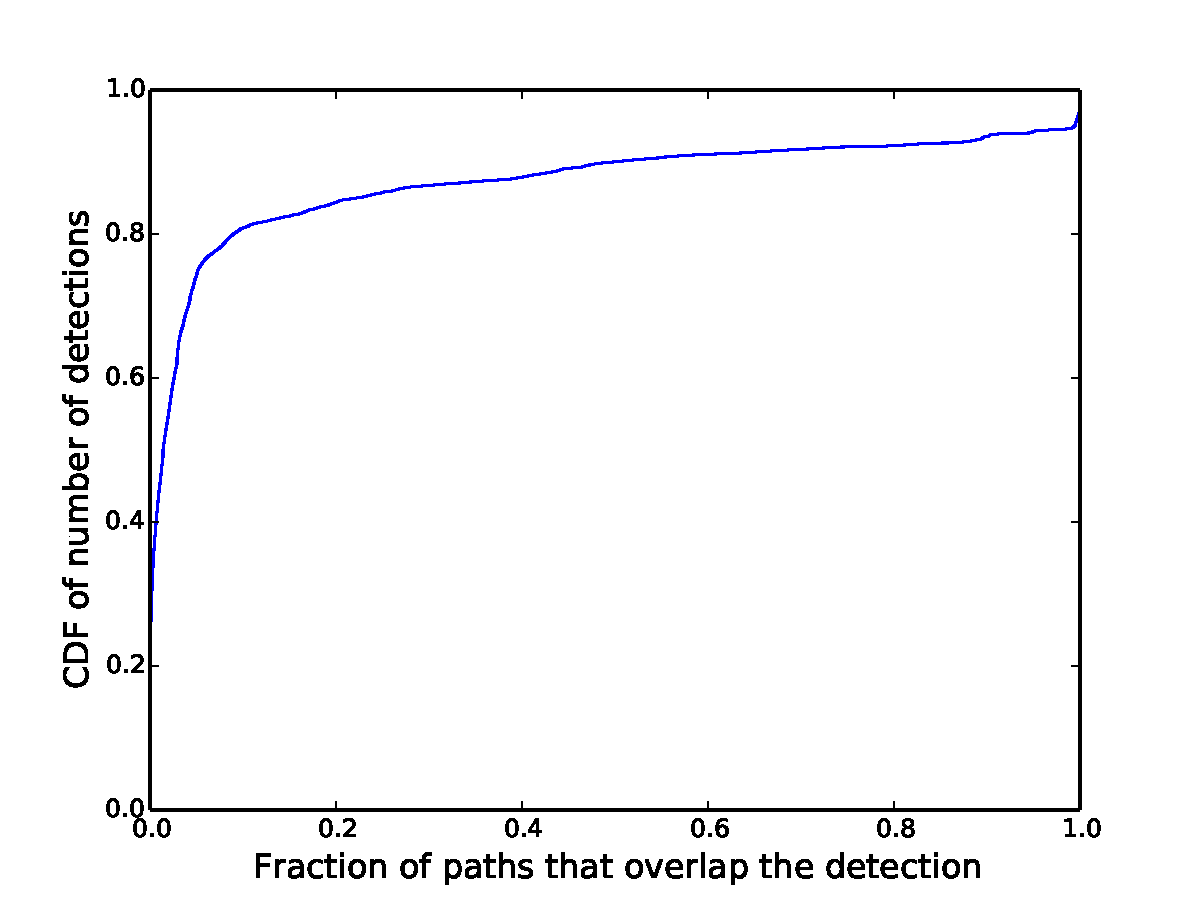
\includegraphics[width=0.8\columnwidth]{figs/patching/routesoverlapping.pdf}
\caption{CDF of detection overlapping with other routes.}
\label{fig:join.acc}
\end{center}
%
\end{figure*}

\begin{figure*}[t]
\begin{center}
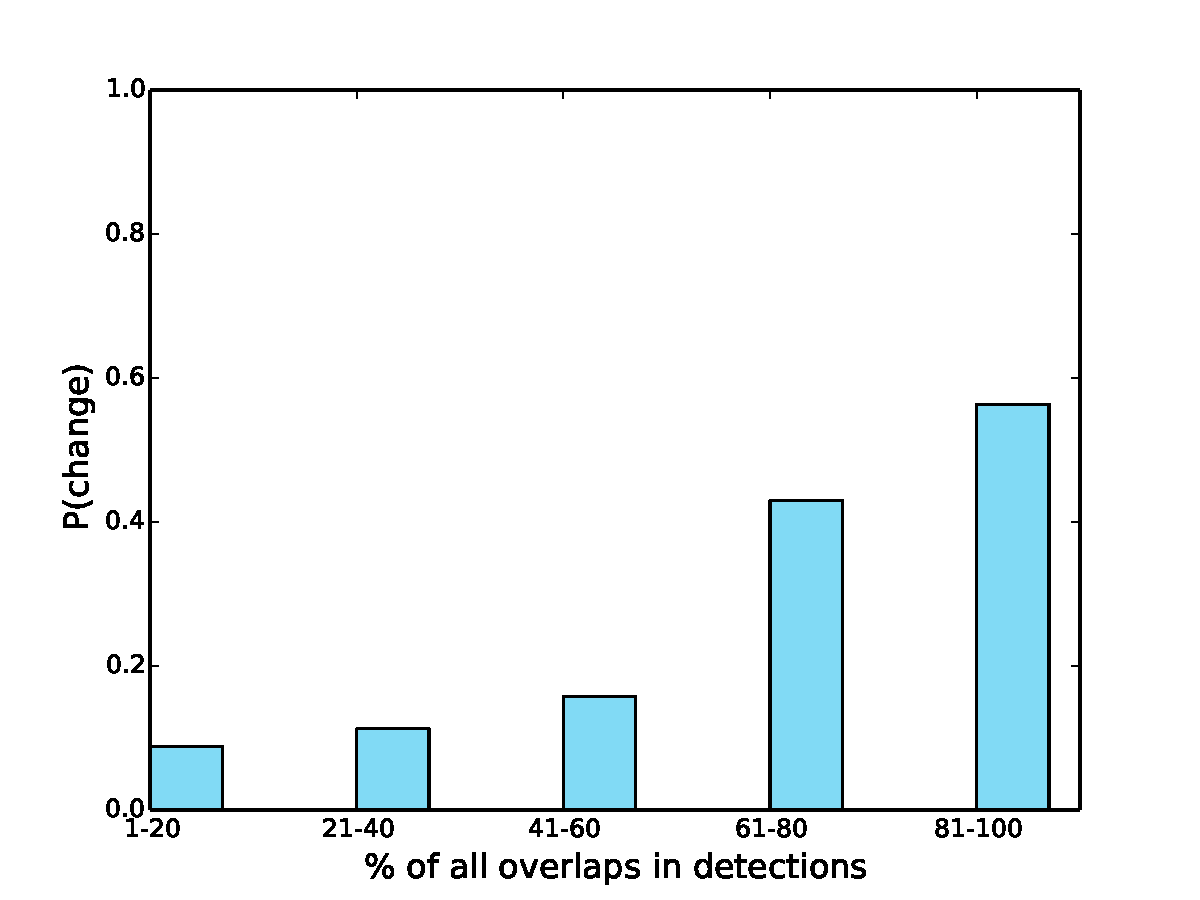
\includegraphics[width=0.8\columnwidth]{figs/patching/probchange.pdf}
\caption{Probability of change given the size of the overlap. }
\label{fig:prob.change}
\end{center}
%
\end{figure*}
%
\begin{figure*}[t]
\begin{center}
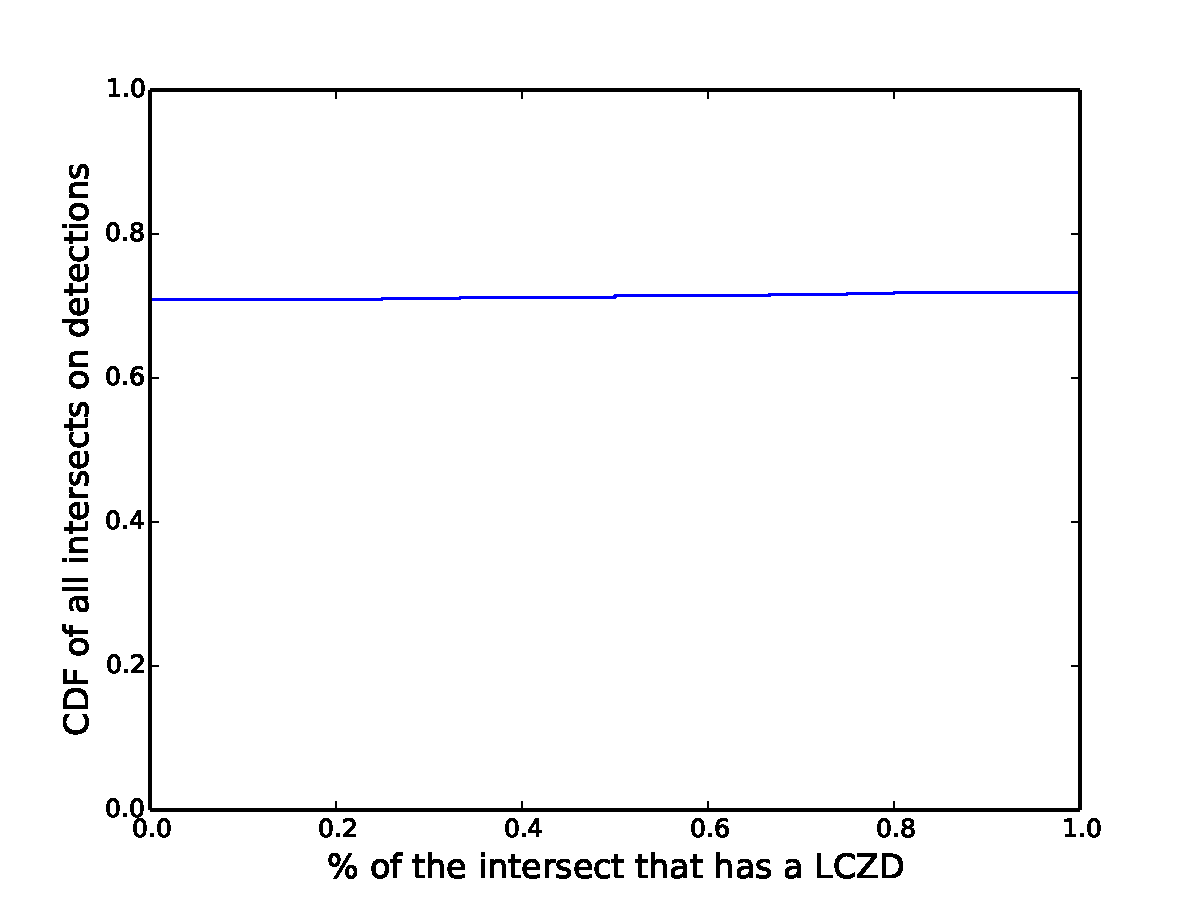
\includegraphics[width=0.8\columnwidth]{figs/patching/overlapcoverage.pdf}
\caption{Probability of a probe detect a candidates that are in a LCZD on other.}
\label{fig:overlap.coverage}
\end{center}
%
\end{figure*}
